In questo capitolo andremo a testare l'applicativo mostrando cosa accade nel
file system ogni volta che PineSU esegue una funzione.
Prenderemo in esame una situazione in cui creeremo due SU, una verrà lasciata aperta,
l'altra verrà prima registrata aperta, poi chiusa e registrata nuovamente, in questo modo
riusciremo anche ad osservare i cambiamenti sull'intero Merkle Calendar.

\section{Prima inizializzazione}

Alla prima apertura di PineSU sulla macchina il processo ci andrà a chiedere
quattro valori: due indirizzi di Wallet Ethereum, la chiave privata del primo dei wallet e,
opzionalmente, la repository Git remota con cui sincronizzare il MerkleCalendar

\section{Creazione delle Storage Unit}

Partiamo definendo il contenuto delle nostre due directory, la prima,
\textbf{\textsf{sample}}, ha questa struttura:
\begin{itemize}
    \itemsep0em
    \item \textsf{sample/graphCreator.js}
    \item \textsf{sample/first/astar.js}
    \item \textsf{sample/first/graph.js}
    \item \textsf{sample/second/priorityQueue.js}
    \item \textsf{sample/second/third/main.js}
    \item \textsf{sample/second/third/vertex.js}
\end{itemize}
Dove \textsf{first} e \textsf{second} sono due subdirectory di \textsf{sample}
e \textsf{third} è una subdirectory di \textsf{second}. \\
I file contenuti sono dei file plain text salvati in formato JavaScript. \\ \\
La seconda directory, \textbf{\textsf{secondSample}}, ha questa struttura:
\begin{itemize}
    \itemsep0em
    \item \textsf{secondSample/esonero1/Immagine.png}
    \item \textsf{secondSample/esonero1/preesonero.pdf}
    \item \textsf{secondSample/esonero1/preesonero.tex}
    \item \textsf{secondSample/esonero2/preesonero2.pdf}
    \item \textsf{secondSample/esonero2/preesonero2.tex}
    \item \textsf{secondSample/esonero3/preesonero3.pdf}
    \item \textsf{secondSample/esonero3/preesonero3.tex}
    \item \textsf{secondSample/esonero3/smith-chart.png}
\end{itemize}

Dove \textsf{esonero1}, \textsf{esonero2} ed \textsf{esonero3} sono tre subdirectory di \textsf{secondSample}.
In questa directory troviamo anche la presenza di file di diversa natura. \\


Per trasformare le directory in Storage Unit posizioniamoci con il terminale all'interno di ognuna,
avviamo lo script di avvio di PineSU e selezioniamo la prima opzione (\emph{Create / Recalculate SU}),
ovviamente il procedimento andrà ripetuto due volte.
Il processo ci chiederà se inizializzare una repository Git e se escludere alcuni file,
procederà poi al calcolo dei vari hash.

\begin{figure}[H]
    \centering
    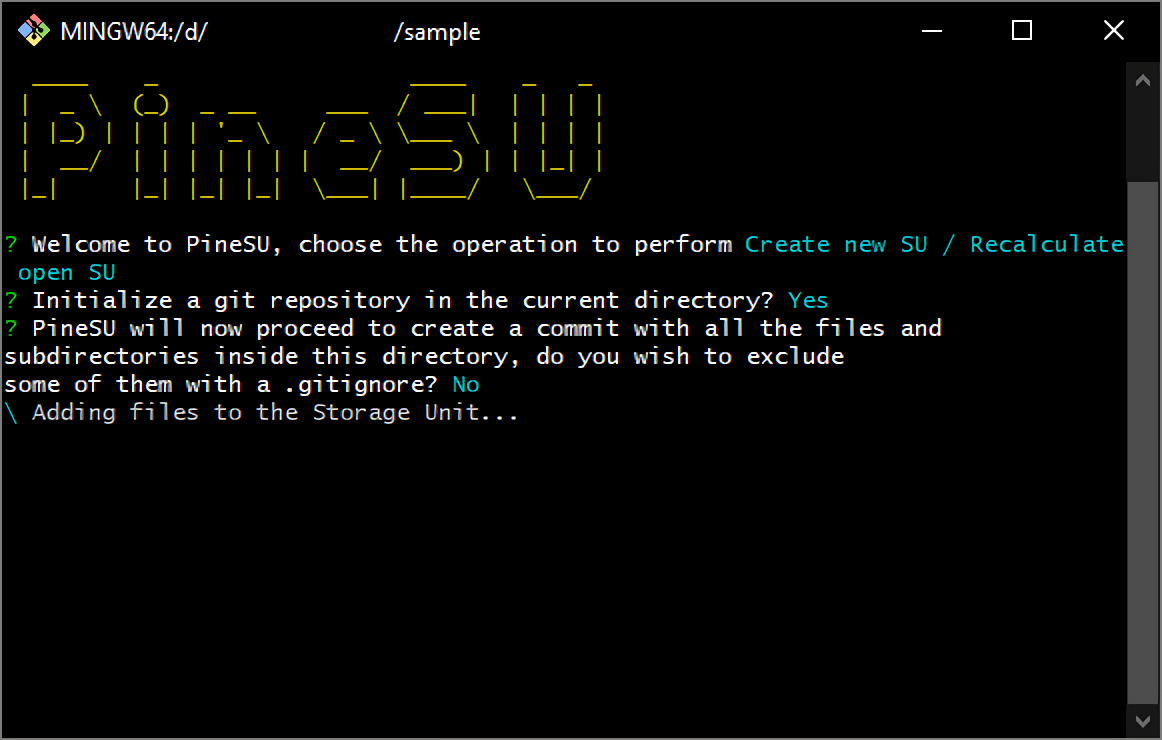
\includegraphics[width=0.9\textwidth]{Figures/calculating}
    \caption{\small{
    L'interfaccia di PineSU durante il calcolo.
    } % end small
    } % end caption
    \label{fi:calc}
\end{figure}


Una volta finito di calcolare ci verranno fatte domande sulla natura della Storage Unit come il suo nome,
la repository remota a cui si sincronizza, la sua descrizione, ecc\dots \\
Finite le domande, l'applicativo ci riporterà al menù principale.

\begin{figure}[H]
    \centering
    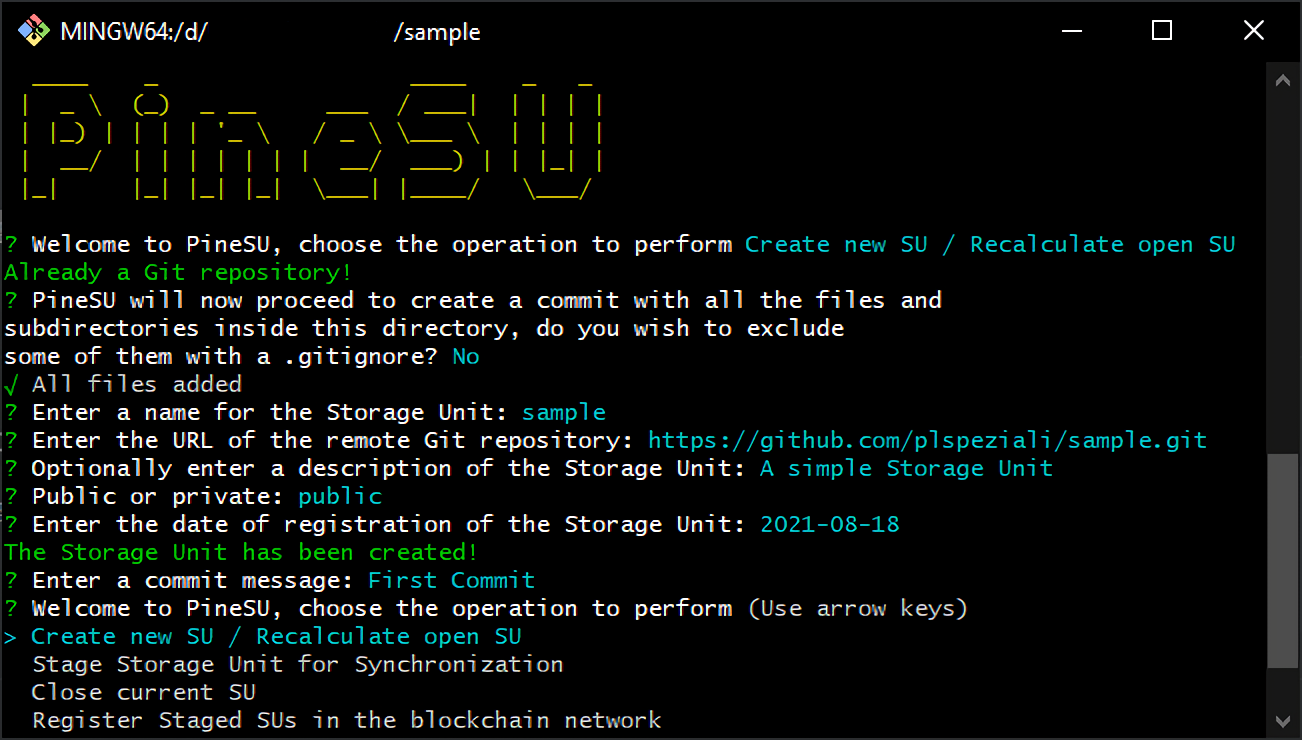
\includegraphics[width=0.9\textwidth]{Figures/doneCalculating}
    \caption{\small{
    L'interfaccia di PineSU appena terminata la fase di creazione.
    } % end small
    } % end caption
    \label{fi:dcalc}
\end{figure}

Al termine di entrambe le elaborazioni sulle due directory avremo alcune nuove aggiunte al loro interno:
una cartella .git (eventualmente, anche un file .gitignore) e un file .pinesu.json, quest'ultimo è
il descrittore JSON in cui sono salvate le informazioni che abbiamo inserito, gli hash calcolati e
lo stato di chiusura. Ecco, ad esempio, il file JSON di \textsf{sample}:

\singlespacing
\begin{lstlisting}[language=json,firstnumber=1]
{"name": "sample",
"remote": "https://github.com/plspeziali/sample",
"description": "A simple Storage Unit",
"visibility": "public",
"date": "2021-08-18",
"owner": "0xCF23544bFC002905532bD86bF647754A84732966",
"hash": "3837ec6fe66032ba593d227ee800a079c61a5853",
"filelist": [
    "first/astar.js:e09deffb3654301a9a8d20acc5a7091cda7039b6",
    "first/graph.js:53982e4feeaf1445434864b409014706e31da1cc",
    "graphCreator.js:c3b4338c33d6ea5a30b31c16defc7661a4ae767b",
    "second/priorityQueue.js:1cb66abaaafd6a7125ab7dac1d7e0fb1860da574",
    "second/third/main.js:1b8dad338691dead8edc66e7c01b8db6d834e3d8",
    "second/third/vertex.js:aa3fa9242ceec7062c7d84764e4068711e53c4e3",
    "first:75d936d52208d14c2cd571e0c595bc29e7d0e3a0",
    "second/third:2ec86afc483f3685893831dfe04b66620be690d2",
    "second:d6e51cdbe8a84cb3ba2c9cfdc2773a96b2401a59"
],
"closed": false }
\end{lstlisting}
\newpage
\onehalfspacing

\section{Staging delle Storage Unit}

A questo punto vogliamo registrare le nostre Storage Unit aperte nella blockchain, 
occorre però prima inserirle negli Storage Group
(in questo caso solo in Open Storage Group).
Per effettuare questa operazione occorre solo selezionare l'opzione apposita (\emph{Stage SU for Synchronization})
in entrambe le directory, nella nostra cartella d'installazione verrà 
aggiornato il file \textsf{merkles/storageGroup.json} con le informazioni delle nostre SU.

\singlespacing
\begin{lstlisting}[language=json,firstnumber=1]
[ {
    "name": "sample",
    "hash": "3837ec6fe66032ba593d227ee800a079c61a5853",
    "path": "D:/sample",
    "closed": false
  },
  {
    "name": "secondSample",
    "hash": "7a61ed5e43cd436fb1f88895625a8193fdb9b3be",
    "path": "D:/secondSample",
    "closed": false
  } ]  
\end{lstlisting}
\onehalfspacing
Questa è la lista delle foglie con cui calcoleremo l'effettivo Merkle Tree di OSG.

\section{Registrazione su Blockchain}
\label{sub:regbc}
Per la registrazione non è necessario posizionarsi in una delle directory delle SU
in quanto quelle da registrare sono già nello Storage Group, ci rimane solo
da selezionare l'opzione apposita (\emph{Register Staged SUs}) per eseguire
con la registrazione, a questo punto lo Storage Group verrà svuotato
e verrà popolato, almeno nel sottoalbero Open, il Merkle Calendar con una foglia
in più e, all'occorrenza, dei nodi interni extra (in caso non fossero state
registrate delle SU in questo mese e anno).

Ovviamente di conseguenza la nuova Merkle Root del Merkle Calendar verrà registrata su
blockchain Ethereum inserendola in un messaggio scambiato tra i due wallet forniti dall'utente,
ciò non è visualizzabile dall'utente a meno che non vada nelle directory delle SU registrate 
in cui potrà trovare un nuovo file \textsf{.registration.json}, esso conterrà informazioni
come la root dello Storage Group in cui è stato registrato, la proof per ricostruire tale root,
l'hash della transazione per recuperarla dalla catena e gli hash dei sottoalberi Open e Closed
del MerkleCalendar nel momento in cui è stato registrato.

\singlespacing
\begin{lstlisting}[language=json,firstnumber=1]
{ "path": "D:/Progetti/Tirocinio/sample",
"root": "e67006f15ecd3fa2719d148be68d3a3242e1be8b",
"proof": [ {
    "right": "7a61ed5e43cd436fb1f88895625a8193fdb9b3be"
} ],
"transactionHash": "0xc56303032[...]2dc87d2e",
"oHash": "e67006f15ecd3fa2719d148be68d3a3242e1be8b",
"cHash": null }  
\end{lstlisting}
\onehalfspacing

\newpage

\section{Verifica d'integrità di una Storage Unit}

A questo punto ci troveremo ad avere Storage Unit USO (Updated Synchronized Open), ciò
significa che ha senso sia effettura verifiche d'integrità avvalendoci della blockchain,
sia esportare sottoinsiemi di file da essa in modo che anche chi reperisce tali file sia
in grado di verificare la loro integrità e la loro registrazione su blockchain.
La verifica può essere fatta selezionando l'opzione \emph{Check SU integrity}
mentre ci si trova nella directory della SU da verificare, il successo o
l'insuccesso ci verranno comunicati su schermo.

\begin{figure}[H]
    \centering
    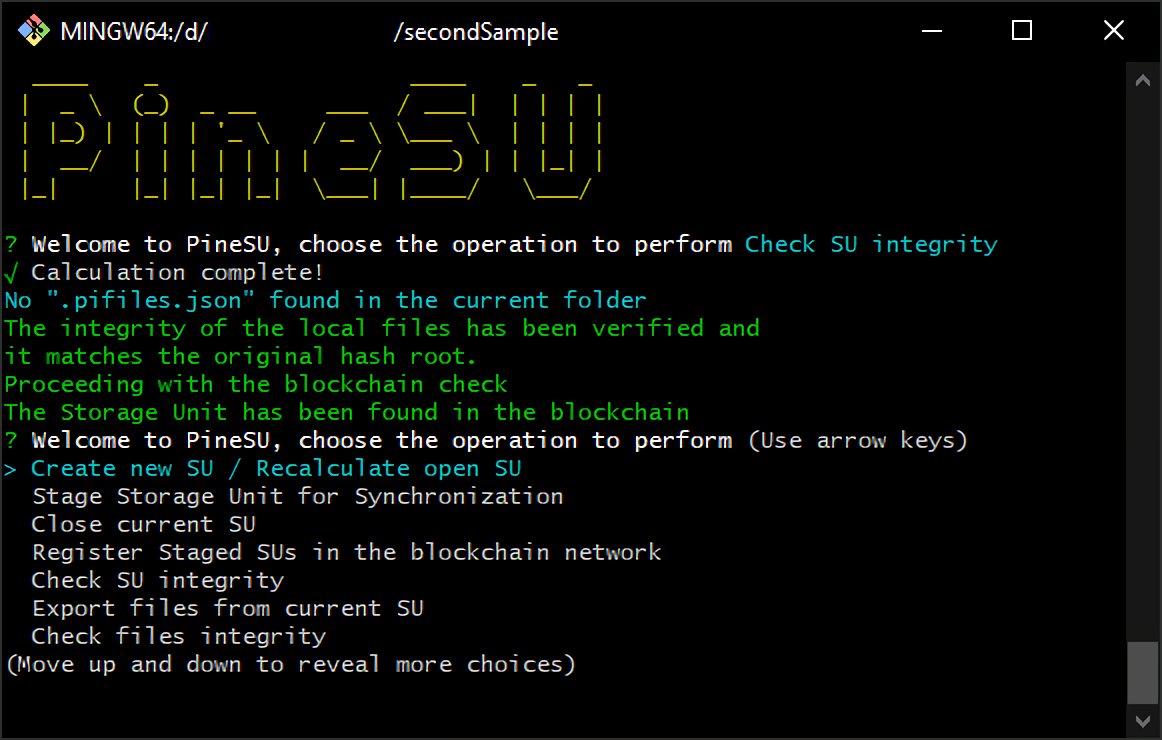
\includegraphics[width=0.9\textwidth]{Figures/verify}
    \caption{\small{
    L'interfaccia di PineSU appena terminata la fase di verifica con successo.
    } % end small
    } % end caption
    \label{fi:ver}
\end{figure}
\newpage

\section{Esportazione di file da una Storage Unit}
\label{sub:exp}
Per quanto riguarda l'esportazione di file, andremo ad eseguirla su \textsf{secondSample}.
Essa viene eseguita selezionando i file da esportare con l'apposita interfaccia
di selezione multipla
\begin{figure}[H]
    \centering
    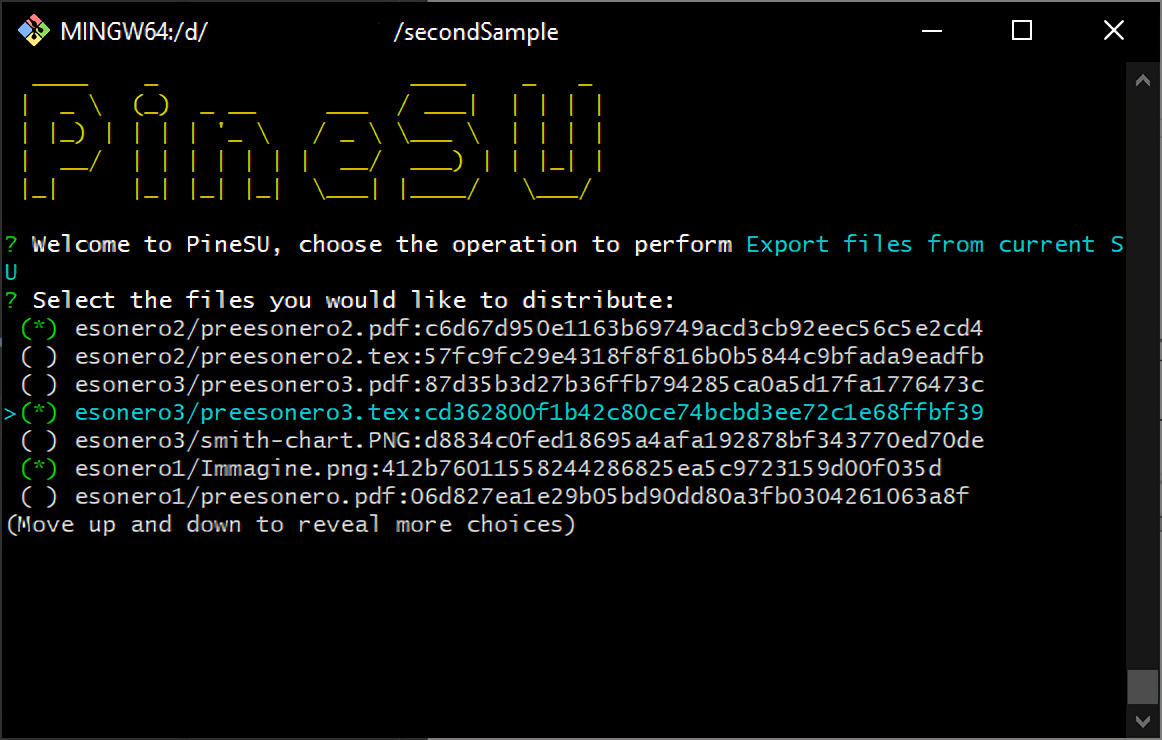
\includegraphics[width=0.9\textwidth]{Figures/export}
    \caption{\small{
    L'interfaccia di PineSU durante un'esportazione.
    } % end small
    } % end caption
    \label{fi:exp}
\end{figure}

In questo caso siamo andati a selezionare \textsf{esonero2/preesonero2.pdf},
\textsf{esonero3/preesonero3.tex} e \textsf{esonero1/Immagine.png}, essi verranno inseriti,
assieme a un file descrittore \textsf{.pifiles.json}, che contiene per ognuno le proof
per ricostruire l'hash della loro SU a partire dai loro hash, e il file \textsf{.registration.json},
in un file ZIP che verrà salvato nella cartella superiore a quella in cui si trovano.

\newpage

\section{Chiusura di una Storage Unit}
Abbiamo già parlato delle implicazioni della chiusura di una Storage Unit, ora descriveremo come
effettivamente può essere realizzata. Di fatto basta eseguire PineSU nella directory della SU e
selezionare l'opzione \emph{Close current SU}, con questa opzione verà aggiunto un commit con un
messaggio particolare, infatti se proveremo a richiudere la stessa Storage Unit, anche se
il file \textsf{.pinesu.json} venisse eliminato, tale commit non ci permetterà di richiuderla
nuovamente.

Procediamo con l'esempio chiudendo \textsf{secondSample} e registrandola nuovamente
su blockchain: in questo caso una foglia verrà aggiunta sia a Closed Storage Group che,
successivamente, al sottoalbero Closed del Merkle Calendar.
Dopo questa operazioni infatti il Merkle Calendar sarà questo:


\singlespacing
\begin{lstlisting}[language=json,firstnumber=1,basicstyle=\small]
"open": [ {
    "name": 2021,
    "hash": "e67006f15ecd3fa2719d148be68d3a3242e1be8b",
    "children": [ {
        "name": 7,
        "hash": "e67006f15ecd3fa2719d148be68d3a3242e1be8b",
        "children": [ {
            "name": "SU of Wed Aug 18 2021 16:00:20",
            "year": 2021,
            "month": 7,
            "day": 3,
            "hour": 16,
            "minute": 0,
            "hash": "e67006f15ecd3fa2719d148be68d3a3242e1be8b"
        } ]
    } ]
} ],
\end{lstlisting}
\newpage\begin{lstlisting}[language=json,firstnumber=18,basicstyle=\small]
"closed" : [ {
    "name": 2021,
    "hash": "7a61ed5e43cd436fb1f88895625a8193fdb9b3be",
    "children": [ {
        "name": 7,
        "hash": "7a61ed5e43cd436fb1f88895625a8193fdb9b3be",
        "children": [ {
            "name": "SU of Thu Aug 19 2021 12:16:36",
            "year": 2021,
            "month": 7,
            "day": 4,
            "hour": 12,
            "minute": 16,
            "hash": "7a61ed5e43cd436fb1f88895625a8193fdb9b3be"
        } ]
    } ]
} ]  
\end{lstlisting}
\onehalfspacing
Come possiamo vedere entrambi i sottoalberi hanno due nodi interni (anno e mese) e la foglia
corrispondente al BSP, quello in Open è stato registrato alla \autoref{sub:regbc}, mentre quello
in Closed è il BSP generato dalla registrazione della SU appena chiusa.

\section{Verifica d'integrità di file esportati}
Avevamo esportato, nella \autoref{sub:exp}, un sottoinsieme dei file di \textsf{secondSample},
una Storage Unit che nel frattempo è mutata chiudendosi, cambiando root e finendo in un
altro sottoalbero di Merkle Calendar, tuttavia l'esportazione era avvenuta quando la SU
era stata registrata già in blockchain come aperta.
Dimostriamo come, nonostante tutto, la verifica su blockchain avvenga senza problemi,
ci basterà infatti posizionarci in una directory arbitraria contenente i file estratti
dal file ZIP e selezionare \emph{Check files integrity} per farsi che il processo svolga i
dovuti controlli e ci comunichi a schermo il successo o l'insuccesso.

\begin{figure}[H]
    \centering
    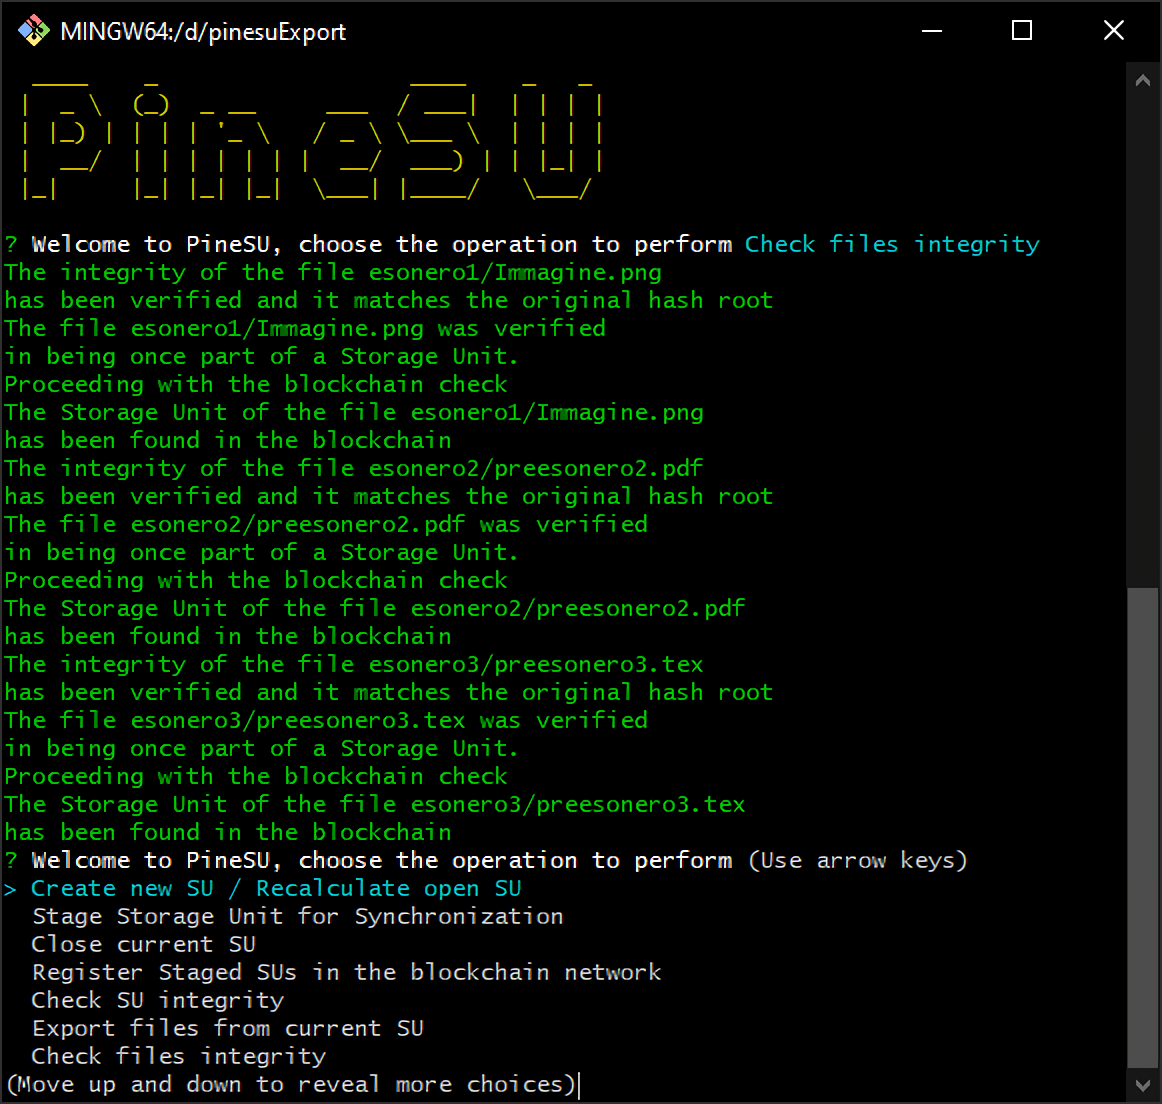
\includegraphics[width=0.9\textwidth]{Figures/verifyFiles}
    \caption{\small{
    L'interfaccia di PineSU durante la verifica dei file esportati da \textsf{secondSample}.
    } % end small
    } % end caption
    \label{fi:vfil}
\end{figure}

Vediamo in Fig.~\ref{fi:vfil} come, per ogni file, viene eseguito un controllo sia locale,
per controllare che non sia stato manomesso, sia remoto, ovvero viene controllato che la SU
di cui lui sostiene di far parte sia stata registrata in blockchain.
